Previous studies of LFU in $b\to s\ell^+\ell^-$ decays have indicated a $\num{3.1}\sigma$ 
deviation from the predictions of the SM \cite{previous_RK}, \cite{previous_RK*}. 
Similar deviations have been observed in measurements of angular observables \cite{angular_1}, 
\cite{angular_2} and in the measurement of branching fractions like 
$\mathcal{B}(B^{(0,+)}\to K^{(+,*0)}\ell^+\ell^-)$ \cite{Branchingfraction}. 
This proceeding discusses the first simultaneous measurement of electron-muon 
universality in the non-resonant regions of the decays $B^+\to K^+\ell^+\ell^-$ and $B^0\to K^{*0}\ell^+\ell^-$.

The observable $r$, which is used to test LFU, is defined as
\begin{equation}
    r_{K,K^*}= 
    \frac{\int_{q_a^2}^{q_b^2}\frac{\mathrm{d}\Gamma(B^{(+,0)}\to K^{(+,*0)}\mu^+\mu^-)}{\mathrm{d}q^2}\mathrm{d}q^2}
    {\int_{q_a^2}^{q_b^2}\frac{\mathrm{d}\Gamma(B^{(+,0)}\to K^{(+,*0)}e^+e^-)}{\mathrm{d}q^2}\mathrm{d}q^2} .
    \label{eqn:single_ratio}
\end{equation}
Theoretically, this ratio is predicted to be $\num{1}$, with corrections at 
the percent level \cite{LU_theo}. This precise prediction is possible because the ratio inherently 
cancels out many of the hadronic uncertainties, which are a common challenge in QCD calculations.
As the decay is depending on the squared dilepton mass $q^2$, the dataset is divided into four $q^2$ regions:
a non-resonant low $q^2$ region ranging from
$\SIrange{0.1}{1.1}{\giga\electronvolt\squared}$,
a non-resonant central region ranging from
$\SIrange{1.1}{6.0}{\giga\electronvolt\squared}$,
and the regions for the $J\!/\!\psi$ resonance ranging from 
$\SIrange{6.0}{11}{\giga\electronvolt\squared}$
and for the $\psi(2S)$ resonance ranging from
$\SIrange{11}{15}{\giga\electronvolt\squared}$.\footnote{In this document, natural units are used where $c=\hbar=1$.}

To mitigate uncertainties arising from efficiencies, the double ratio 
\begin{equation}
    R_{K,K^*}= 
    \frac{\frac{N}{\epsilon}(B^{(+,0)}\to K^{(+,*0)}\mu^+\mu^-)}
    {\frac{N}{\epsilon}(B^{(+,0)}\to K^{(+,*0)}e^+e^-)}
    \underbrace{\frac{\frac{N}{\epsilon}(J\!/\!\psi(e^+e^-))}{\frac{N}{\epsilon}(J\!/\!\psi(\mu^+\mu^-))}}_{(r^K_{J\!/\!\Psi})^{-1}}
    \label{eqn:double_ratio}
\end{equation}
is defined.
In this equation, $N/\epsilon$ represents the yield of the process, corrected by 
the efficiency. The ratio in the resonant region $r^K_{J\!/\!\psi}$ is known to be 
$\num{1}$ \cite{AULCHENKO2014227}. Due to the complexity involved in estimating 
efficiencies, the double ratio provides a more stable measure against systematic 
uncertainties.

The Large Hadron Collider beauty experiment (LHCb) is one of the four major experiments 
at the Large Hadron Collider (LHC) at CERN. It is designed to conduct high-precision 
measurements of particle decays involving $b$ and $c$ quarks. Given that $b\bar{b}$ pairs 
are boosted in the beam direction, the detector is constructed as a single-arm forward 
spectrometer. \cite{LHCb}

The LHCb trigger system for Run 1 and 2 is a three-level system designed to select relevant events from 
the multitude of proton-proton collisions. The first level, known as the Level-0 trigger 
(L0), is hardware-based and reduces the event rate based on information from the calorimeter 
and muon systems. The subsequent levels, HLT1 and HLT2, are software-based. HLT1 applies 
fundamental conditions for partially reconstructed events, while HLT2 utilizes complete 
reconstruction of candidates and employs topological information to further reduce the 
data volume. \cite{trigger}

The track reconstruction process is carried out using the Vertex Locator (VELO), which 
captures the particle tracks very close to the point of collision. This process is further 
facilitated by four additional tracking stations, which provide more data points for a 
comprehensive and accurate reconstruction of the particle paths.

Particle identification (PID) at LHCb is carried out using information from several 
sub-detectors. The RICH (Ring Imaging Cherenkov) detectors provide PID information by 
measuring the Cherenkov angle of charged particles. The calorimeter system is utilized 
to identify photons, electrons, and hadrons, and to measure their energies. The muon 
system is employed to identify muons. The performance of the PID system is crucial for 
numerous analyses at LHCb, including the measurement of LFU in $b\to s\ell\ell$ 
decays. \cite{LHCb}

The reconstruction of decay in the electron and muon channels presents varying levels of 
complexity, primarily due to three factors. First, electrons emit bremsstrahlung, which 
can lead to inaccurate measurements of their energy or momentum. This necessitates a wider 
fit range, which, while it increases sensitivity to peaking structures, also 
introduces more background into the data. Furthermore, the lineshapes in the data become 
dependent on bremsstrahlung, requiring additional considerations in the data interpretation 
process. The electrons are categorized in three bremsstrahlung categories based on the 
number of emitted photons. For each categorie an individual particle density function (PDF) 
is developed. These individual PDFs are then amalgamated in a ratio that reflects the observed 
frequency of bremsstrahlung categories, thereby creating an aggregate PDF for fitting to the 
data.
Second, the electronic calorimeter's energy resolution is characterized 
by substantial uncertainties. The poor spatial resolution of the calorimeter also complicates 
the allocation of bremsstrahlung photons to the respective electron. This results in a 
bremsstrahlung recovery efficiency of $\mathcal{O}(\SI{50}{\%})$.
Third, the efficiency of the L0 trigger for muons is higher than for electrons, resulting 
in a selection effect of approximately $1/3$ when comparing $\text{L0}e$ to $\text{L0}\mu$.
These elements collectively contribute to differences in the efficiencies in the two channels. 

To neutralize the varying efficiencies of the L0 trigger, one can employ events that are 
triggered independently of the signal, known as Trigger Independent Signal (TIS) events. 
In these instances, the $B$ candidate does not influence the trigger, thereby ensuring that 
the efficiencies between the electron and muon modes are balanced.

The simulations used for the analysis were specifically generated for each data-taking period 
to accurately represent the respective conditions. These simulations take into account a multitude 
of factors that could influence the data, including the specific properties of the detector and 
the environmental conditions during data collection. A crucial aspect of the simulations is the 
modeling of final state radiation, for which the \texttt{PHOTOS} \cite{PHOTOS} program is utilized. 
\texttt{PHOTOS} is a specialized tool developed to accurately simulate the effects of bremsstrahlung in 
final state particle production. By combining these detailed simulations with the data from the 
experiments, a precise analysis of the decay processes can be conducted.

To enhance the signal-to-background ratio, two multivariate classifiers are employed. The 
first classifier is designed to distinguish the signal from the combinatorial background, 
which is composed of randomly assembled tracks. This classifier utilizes information about 
the kinematics and geometry of the final state, as well as details about the vertex and the 
quality of the vertex fit.

The second classifier is used to differentiate between the signal and partially reconstructed 
background. These are processes with additional particles $X$ in the final states, such as 
$B\to K \ell^+\ell^- X$. If the particles $X$ are not correctly reconstructed, the process may be mistakenly 
identified as $B \to K \ell^+\ell^-$. This classifier also uses kinematic and geometric features of 
the final states, but additionally, it incorporates information about the spatial and kinematic 
isolation of the final state particles in relation to other reconstructed particles.

To avoid bias, a $k$-folding validation is implemented. Both classifiers are optimized 
simultaneously for each lepton flavor, $q^2$ region, and data-taking period separately.

To mitigate the effects of partially reconstructed background, the momentum of the 
dielectron system, $\vec{p}(e^+e^-)$, is corrected as
\begin{equation}
    \vec{p}_\text{corr}(e^+e^-)=\vec{p}(e^+e^-)\cdot\frac{p_\text{T}(h)}{p_\text{T}(e^+e^-)}.
\end{equation}
In this equation, $p_\text{T}(h)$ represents the transverse momentum of the hadron. 
Subsequently, the corrected mass is computed using the corrected momentum and the 
momentum of the hadron, $p_h$
\begin{equation}
    m_\text{corr}=|\vec{p}_\text{corr}(e^+e^-)+\vec{p}_h|.
\end{equation}
The distributions of signal and background in $m_\text{corr}$ separate to such an extent 
that a cut can be applied. After the selection of $m_\text{corr}$ all backgrounds with two 
or more missing hadrons are removed from the data.

The simulations utilized in the analysis are calibrated to accurately represent the difference 
between electrons and muons. To achieve this, weights are computed via 
$w_i=\epsilon_\text{data}/\epsilon_\text{Simulation}$ for the $J\!/\!\psi$ resonant decays in a chain 
for each calibration category $i$. 
The corrections are applied across multiple areas. For instance, the PID is adjusted to ensure 
that the simulation correctly identifies particles as electrons or muons. The tracking of 
particles in the simulation is also corrected to match the real-world data, a process referred 
to as Tracking (TRK) correction.
To accurately represent the kinematics of $B$ mesons and the multiplicity of events, adjustments 
are made under the category of $B$ kinematics and event multiplicity (BKIN\&MULT). The simulation's
representation of the hardware trigger's efficiency in real-world data is calibrated under the 
L0 correction.
Similarly, the HLT correction is applied to ensure the simulation accurately represents the software 
trigger. The $B$ decay vertex reconstruction (RECO) correction ensures that the simulation accurately 
represents the reconstruction of the $B$ decay vertex.
Lastly, the $q^2$ resolution and bin-migration (RES) correction is applied to adjust the simulation 
accurately represent the resolution of $q^2$ and the migration of bins. These corrections are crucial 
in ensuring that the simulations provide an accurate representation of the real-world data and thus, 
reliable results.

The effects of these corrections for $B^+\to K^+e^+e^-$ are illustrated in figure \ref{fig:weights}. 
Although the figure specifically depicts the scenario for $B^+\to K^+e^+e^-$, the behavior for 
$B^0\to K^{*0}e^+e^-$ is analogously observed. It is evident that the double ratios $R$ are 
significantly less influenced by the corrections than the single-ratio $r^{K^*}_{J\!/\!\psi}$. 
The single-ratio efficiency changes by $\SI{25}{\%}$, while all double ratio efficiencies are 
altered by at most $\SI{5}{\%}$. This demonstrates that the double ratio is a more robust observable 
than the single-ratio when it comes to uncertainties in the efficiencies.

\begin{figure}
    \centering
    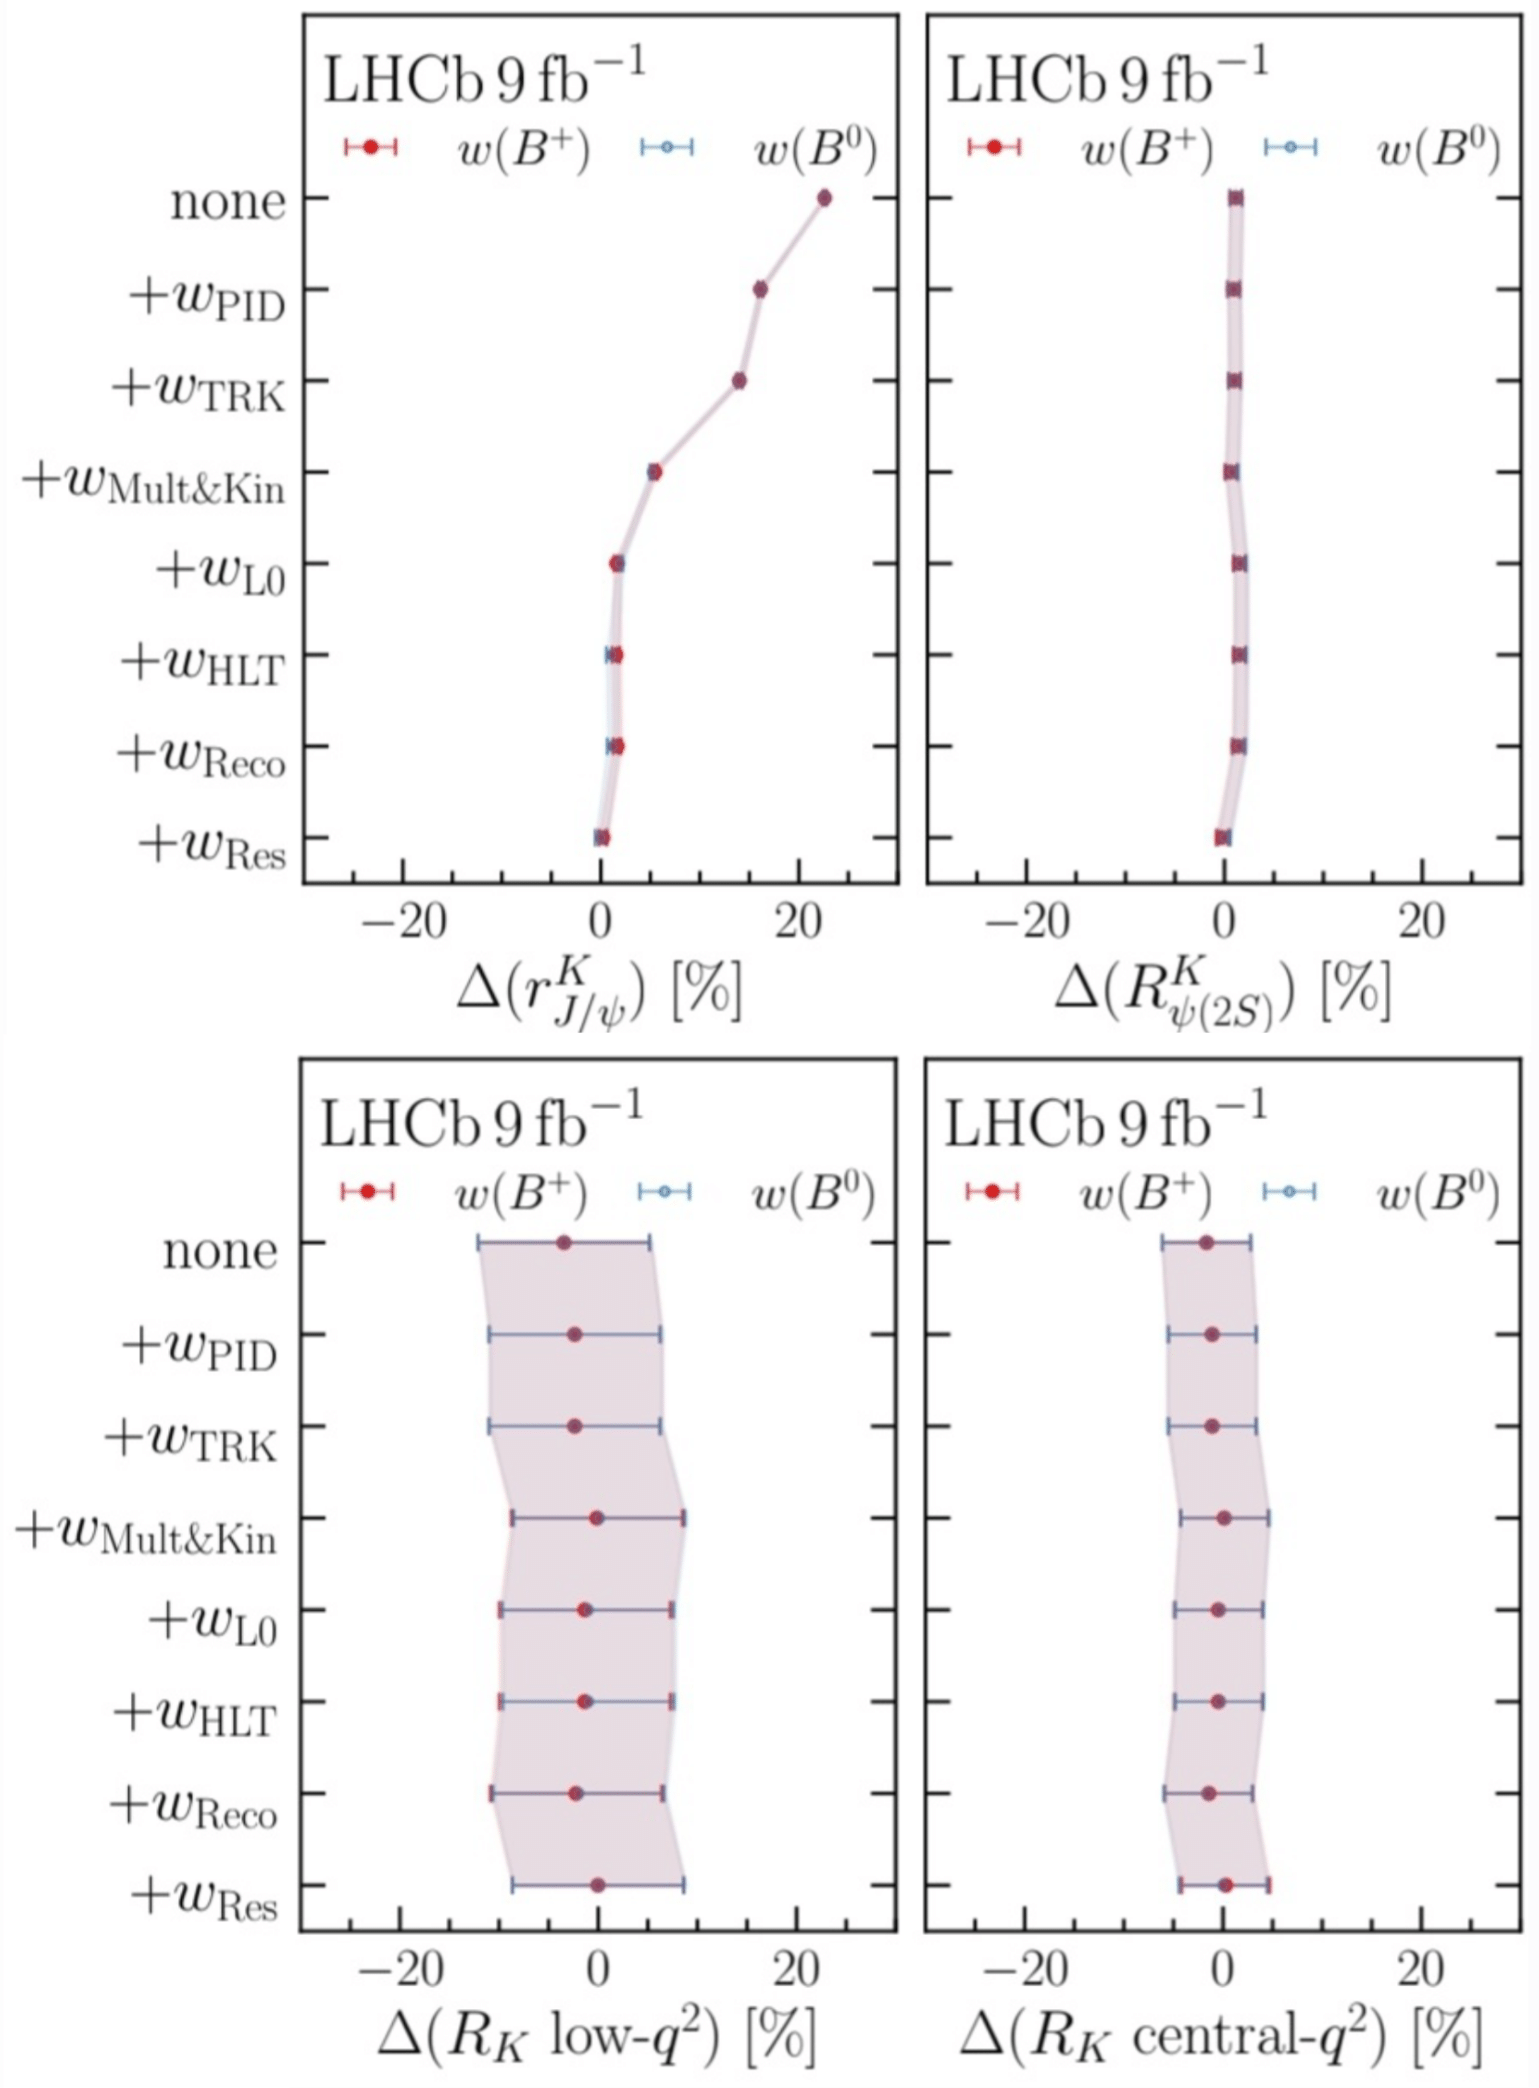
\includegraphics[width=0.84\linewidth]{figures/weights_cut.png}
%    \caption{Variation of the efficiencies regarding to the corrections for the ratios (left to right):
%    $r^{K}_{J\!/\!\psi}$, $R^{K}_{\psi(2S)}$, $R_{K}$ in the low- and central $q^2$ region (top row) 
%    and the corresponding ratios for $K^*$ (bottom row). %The calibration of the simulation, which uses 
%    %$B^0$ and $B^+$ chains for sequential calibration weights, is displayed and shows a near-identical match 
%    \cite{lhcbcollaboration2022test}.}
    \caption{Variation of the efficiencies regarding to the corrections for the ratios (left to right):
    $r^{K}_{J\!/\!\psi}$, $R^{K}_{\psi(2S)}$ (top row) and $R_{K}$ in the low- and central $q^2$ region (bottom row).
    \cite{lhcbcollaboration2022test}.}
    \label{fig:weights}
\end{figure}
To cross-check all previous steps the ratios $r^{K^{(*)}}_{J\!/\!\psi}$ and 
${R^{K^{(*)}}_{\psi(2S)}=r^{K^{(*)}}_{\psi(2S)}/r^{K^{(*)}}_{J\!/\!\psi}}$ 
are calculated. As expected both are compatible with $\num{1}$.

The calculation of the double-ratio is performed by a simultaneous maximum-likelihood 
fit to the invariant mass distribution of the reconstructed $B^0$ and $B^+$ in the 
non-resonant $q^2$ regions and the $J\!/\!\psi$ resonance. 

In the muon mode, the invariant mass distribution consists only of the signal and 
combinatorial background. 
In the case of the electron, the distribution is much more complicated due to 
residual misidentified hadronic decays and partially reconstructed background. 
Additionally, there are contributions from the resonant $J\!/\!\psi$ decay that extend 
into the central $q^2$ region. 
The signal and these additional components are modeled using various techniques, 
including kernel-density estimators derived from simulated data.

A novel approach to understanding the background arising from misidentified 
electrons is developed in this analysis. After the selection process, the remaining 
misidentified electron background is determined by inverting the PID requirements 
on one or both electrons. The electron-candidates are then categorized as kaon- or 
pion-like using a kaon ID classifier. This information is used to predict and model 
the background shape.
This misidentified background was not included in previous mass fits and therefore
leads to different results of $R_K$ and $R_K^*$ \cite{previous_RK}, \cite{previous_RK*}.

The combinatorial background is modeled as a decreasing exponential function. 
Its distortion by the corrected mass and the selection criteria for partially 
reconstructed events is parametrized by a function derived from background data. 
The fit for $B^+\to K^+e^+e^-$ in the central $q^2$ region is illustrated in 
figure \ref{fig:fits}. 
While the figure shows the central $q^2$ region for $B^+\to K^+e^+e^-$, the low 
$q^2$ region and $B^0\to K^{*0}e^+e^-$ fits are done simultaneously but not depicted 
here.
The signal yield is then used to calculate 
the double-ratio using the definition \eqref{eqn:double_ratio}.

\begin{figure}
    \centering
    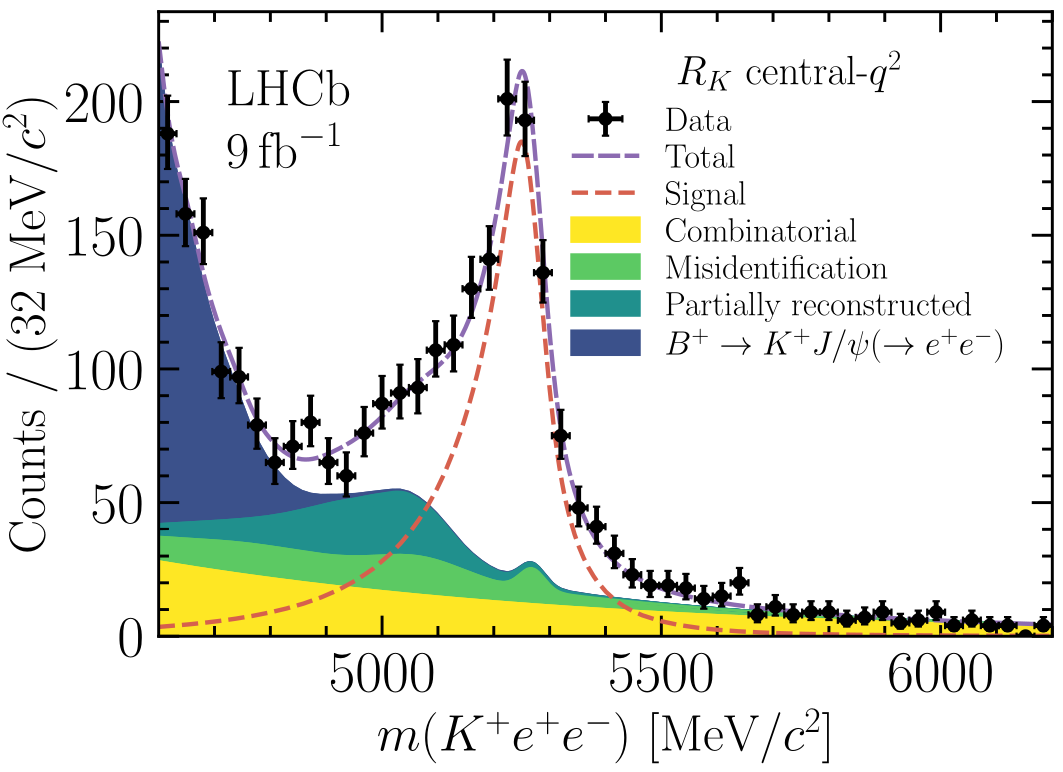
\includegraphics[width=0.84\linewidth]{figures/fits_3.png}
%    \caption{Maximum-likelihood fit of the invariant mass distributions in the central $q^2$ (upper) and lower $q^2$ (lower) region for the non-resonant decays $B^+\to K^+e^+e^-$ (left) and $B^0\to K^{*0}e^+e^-$ (right) \cite{lhcbcollaboration2022test}.}
    \caption{Maximum-likelihood fit of the invariant mass distributions in the central $q^2$ region for the non-resonant decays $B^+\to K^+e^+e^-$ \cite{lhcbcollaboration2022test}.}
    \label{fig:fits}
\end{figure}

The results obtained for the observables are
\begin{align*}
    \text{low $q^2$} 
    &\left\{
    \begin{aligned}
        &R_{K}  \!\!\!\!\!\!\!&&=\, 0.994 \,\substack{+0.090 \\ -0.082}\,\text{(stat)}\,\substack{+0.029 \\ -0.027}\,\text{(syst)}\\
        &R_{K^*}\!\!\!\!\!\!\!&&=\, 0.927 \,\substack{+0.093 \\ -0.087}\,\text{(stat)}\,\substack{+0.036 \\ -0.035}\,\text{(syst)}
    \end{aligned}
    \right. \\
    \text{central $q^2$} 
    &\left\{
    \begin{aligned}
        &R_{K}  \!\!\!\!\!\!\!&&=\, 0.949 \,\substack{+0.042 \\ -0.041}\,\text{(stat)}\,\substack{+0.022 \\ -0.022}\,\text{(syst)}\\
        &R_{K^*}\!\!\!\!\!\!\!&&=\, 1.027 \,\substack{+0.072 \\ -0.068}\,\text{(stat)}\,\substack{+0.027 \\ -0.026}\,\text{(syst)}.
    \end{aligned}
    \right.
\end{align*}
At a first approximation, these observables are uncorrelated.

The dominant systematic uncertainties in modeling the invariant mass distribution 
modeling arise from the data-driven modeling of misidentified backgrounds, 
varying between $\SI{2.0}{\%}$ and $\SI{2.5}{\%}$ based on the observable. 
Another significant uncertainty is linked to the stability of the 
single-ratios $r^{K^{(*)}}_{J\!/\!\psi}$, depending on the decay's kinematics 
and geometry. Excluding the low $q^2$ region for $R_{K^*}$, this uncertainty contributes 
significantly less than that from misidentified backgrounds. Overall, statistical 
uncertainties dominate the uncertainty of the results.

